\documentclass[12pt]{article}

% packages
\usepackage{sbc-template}
\usepackage{graphicx,url}
% \usepackage[brazil]{babel}   references and labels in English
\usepackage[utf8]{inputenc}  
\usepackage{lipsum}
\usepackage{caption} % Subfigure package
% \usepackage{subcaption}
\usepackage{graphicx}
\usepackage{listings}
\usepackage{xcolor}

% gro language definition
\definecolor{COLOR_COMMENTS}{RGB}{16, 97, 35}
\lstdefinelanguage{GROLANG}{
    morekeywords={include,program,rate,ecoli},
    sensitive=false,
    morecomment=[l]{//},
    morestring=[b]",
}
\lstdefinestyle{GROSRC}
{
  language     = GROLANG,
  basicstyle   = \footnotesize,
  commentstyle = \color{COLOR_COMMENTS},
  frame=single,
  tabsize=2,
  framexleftmargin=8pt,
}

% info
\sloppy
\title{Albi:\\ A Gro compiler to the SBML standard}
\author{Alek Frohlich\inst{1}, Gustavo Biage\inst{1}}
\address{Departamento de Informatica e Estatística – Universidade Federal de Santa Catarina \\
Florianopolis – SC – Brazil
  \email{\{alek.frohlich,gustavo.c.biage\}@grad.ufsc.br}
}

% paper
\begin{document}
\maketitle

%       => the Growth of the area leads to the development of multicellular devices
%       => gro is well suited for this purpose
%       => however it isn't ready for compatibility
%       => introduce the objective of making it compatible
\begin{abstract}


    The Growth of research areas such as synthetic biology and systems biology leads to an increased willing to develop new, larger mathematical models to describe complex biological behavior. In order to enable natural flow of development of those models, scientists must have access to tools which increase the level of abstraction and enable reuse of biological components. Increased efforts are being put on solving these two problems. The present work tackles those problems by interfacing the existing programming language Gro with SBML for model interchangeability and ease of model representation.


\end{abstract}

%       => what does albi fix that libSBML does not?
%       => what are the reasons we chose Gro as albi's primary language?
%       => what are the disadvantages of the Gro simulator
%       => what are the advantages of having the SBML model for a Gro program?
%       => introduce following sections
\section{Introduction}


    Even though a Systems Biology Markup Language API library (LibSBML) has already been developed \cite{Bornstein2008}, it only ought to be useful in cases where a new model is to be developed. In cases where there is a preexisting model, the availability of an SBML library doesn't help much since the previous model would have to be entirely rewritten to fit the API. Instead, the present work proposes a language parser that generates SBML code from previously built Gro models. Gro is a language for programming, modeling, specifying and simulating the behavior of cells in Growing micro colonies of microorganisms \cite{Jang2012}. It has been made the primary source of the parser considering it has many interesting syntactical constructs such as rate statements, program definitions and bacterial instantiation which can be neatly represented, respectively, in SBML documents as reactions, local name spaces and compartments.
    
    As language support goes, Gro is still tightly coupled with it's original simulator. Although the simulator has recently undergone big improvements in the sense that simulations behave more realistically \cite{Gutirrez2017}, it doesn't change the fact that using it is the only available way to validate Gro models. This hinders the reproducibility of experiments built with the language. SBML models, on the other hand, are supported by more than 100 software systems \cite{Hucka2007}, making them more likely to be verified and reused.
    
    If Gro code were to be translated into SBML, the document could be further preserved as an entry in BioModels. BioModels is a database of curated SBML and CellML models maintained with the intent of providing researches with models related to a particular disease, biological process or molecular complex \cite{LeNovere2006}. Having a model curated is an even stronger guarantee of trustworthiness since the process is done manually for each model \cite{LeNovere2006}: Newly submitted models go through a series of syntactical analysis to confirm that they are valid syntactically and well formatted; The model is then numerically verified against the results claimed by the authoring paper; Finally, the validated model gets manually annotated and cross-linked to facilitate later search for it.
    
    The rest of the paper is structured as follows: In Sect. 2, we introduce the language parser and explain the process of converting gro files to SBML models from start to end; In Sect. 3, we compile a Gro implementation of the repressilator, a synthetic oscillator, to equivalent SBML and then simulate it on COPASI, a pathway simulator \cite{Hoops2006}; In Sect. 4, we summarize what's been done and compare it with goals laid out at the start; In Sect. 5 we conclude by presenting possible extensions of the current work.
    
    
\section{Architecture}

%       => present Albi's syntax
%       => the transition between single cell systems biology to multi cell ??
%       => examples of generated SBML
\subsection{The parser}
    
    Currently, the parser only recognizes a subset of gro's syntax. Valid programs are constituted by global variable declarations, program definitions and E. coli instantiations. Parameters, messages and guarded statements are also recognized as valid syntax, however no semantic value is assigned to them as control statements and user interaction function do not make sense in the context of an SBML model. Below is the gro code for the Repressilator, whose mathematical model shall be explained in the next section.
    
    % repressilator source code
    \input{repressilator_gro_src.tex}
    
    This gro model of the repressilator is then compiled down to the intermediate representation accepted by the code generation framework Tellurium.
    
    \begin{lstlisting}[style=GROSRC]
        beta = 0.2000;
        n = 2.0000;
        alfa0 = 0.0300;
        compartment ECOLI0
        ECOLI0 = 1.0
        var ECOLI0_prog_m1 in ECOLI0
        ECOLI0_prog_m1 = 0.0000
        var ECOLI0_prog_m2 in ECOLI0
        ECOLI0_prog_m2 = 0.0000
        var ECOLI0_prog_m3 in ECOLI0
        ECOLI0_prog_m3 = 0.0000
        var ECOLI0_prog_p1 in ECOLI0
        ECOLI0_prog_p1 = 0.0000
        var ECOLI0_prog_p2 in ECOLI0
        ECOLI0_prog_p2 = 5.0000
        var ECOLI0_prog_p3 in ECOLI0
        ECOLI0_prog_p3 = 15.0000
        -> ECOLI0_prog_p3;(((beta)*(ECOLI0_prog_m3))-((beta)*(ECOLI0_prog_p3)));
        -> ECOLI0_prog_p2;(((beta)*(ECOLI0_prog_m2))-((beta)*(ECOLI0_prog_p2)));
        -> ECOLI0_prog_p1;(((beta)*(ECOLI0_prog_m1))-((beta)*(ECOLI0_prog_p1)));
        -> ECOLI0_prog_m3;(((alfa)/((1.0000)+((ECOLI0_prog_p2)^(n))))-(ECOLI0_prog_m3));
        -> ECOLI0_prog_m2;(((alfa)/((1.0000)+((ECOLI0_prog_p1)^(n))))-(ECOLI0_prog_m2));
        -> ECOLI0_prog_m1;(((alfa)/((1.0000)+((ECOLI0_prog_p3)^(n))))-(ECOLI0_prog_m1));
        -> ECOLI0_prog_m3 + ECOLI0_prog_m2 + ECOLI0_prog_m1;(alfa0);
    \end{lstlisting}
    
\subsection{The Tellurium framework}
    \lipsum[1]

\subsection{libSBML}
    \lipsum[1]
    
\section{Study case: The Repressilator}

The study case for this articles aims to identify and explain subtle differences in how simulations occurs and the benefits of each, also to explore the applicability of the Gro to SBML parser and establish a certainty of both models, to achieve such goal we will set off from the mathematical model presented in octave, later extract the elements and construct the Gro algorithm structure. 

From the algorithm we should make use of the parser and generate a SBML standard file to be simulated in COPASI software presenting the same behaviour and mathematical model, primarily the derivatives. Even though, if both deterministic simulations achieved present similar comportment, it is still necessary to conclude that the Gro delivers the same conduct.

\subsection{Mathematical Model}

% Introduz o modelo aqui

%derivatives

$\frac{d}{dt}m_{1}(t) = \alpha_{0} + \frac{\alpha}{1 + [p_{3}(t)]^{n}} - m_{1}(t)$

$\frac{d}{dt}m_{2}(t) = \alpha_{0} + \frac{\alpha}{1 + [p_{1}(t)]^{n}} - m_{2}(t)$

$\frac{d}{dt}m_{3}(t) = \alpha_{0} + \frac{\alpha}{1 + [p_{2}(t)]^{n}} - m_{3}(t)$

$\frac{d}{dt}p_{1}(t) = \beta{m_{1}}(t) - \beta{p_{1}}(t)$

$\frac{d}{dt}p_{2}(t) = \beta{m_{2}}(t) - \beta{p_{2}}(t)$

$\frac{d}{dt}p_{3}(t) = \beta{m_{3}}(t) - \beta{p_{3}}(t)$ 

In the process of obtaining the the oscillatory comportment, it is needed to establish a bi-stability, the information obtained is the manners of concentrations rapidly changing from a high "voltage" to a low "voltage", in the computer science perspective, which in this case the binary states are defined by the protein and molecules level of concentration. The initial concentrations values for this model is $m_{1} = m_{2} = m_{3} = 0$, $p1 = 0$, $p_{2} = 5$ and $p_{3} = 15$; the parameters are $n = 2$, $\alpha = 298.2$, $\alpha_{0} = 0.03$ and $\beta = 0.2$, of the same nature as the ones accomplished in the simulation graphs. \cite{ingalls2013mathematical}.

% Phase plane
\begin{figure}[h]
    \centering
    \includegraphics[scale = 0.5]{apagar.png}
    \caption{Caption}
    \label{fig:phase_plane_repressilator}
\end{figure}

When using deterministic simulations for a mathematical model in a hard to predict experiment, depending on how sensible to variables changes the model is, it can have a different performance than the one expected, that is why in stochastic simulations the frequency of the clock varies. The repressilator, in particular, oscillation occurs very close to a region of stable steady state, as it can be observed in figure \ref{fig:phase_plane_repressilator}, therefore, of the many simulations to determine the behaviour, the outliers or unexpected presentation could manages to fall into a steady state where no more oscillation occurs, in a way that based on how the derivatives achieved the value of 0 it can no longer leave that state, even through outside impact. What should be concluded by it, is that this model can come to stop the oscillations and and start it again if observed multiple times by a long period of time.

% Oscillation
\begin{figure}[ht]
\centering
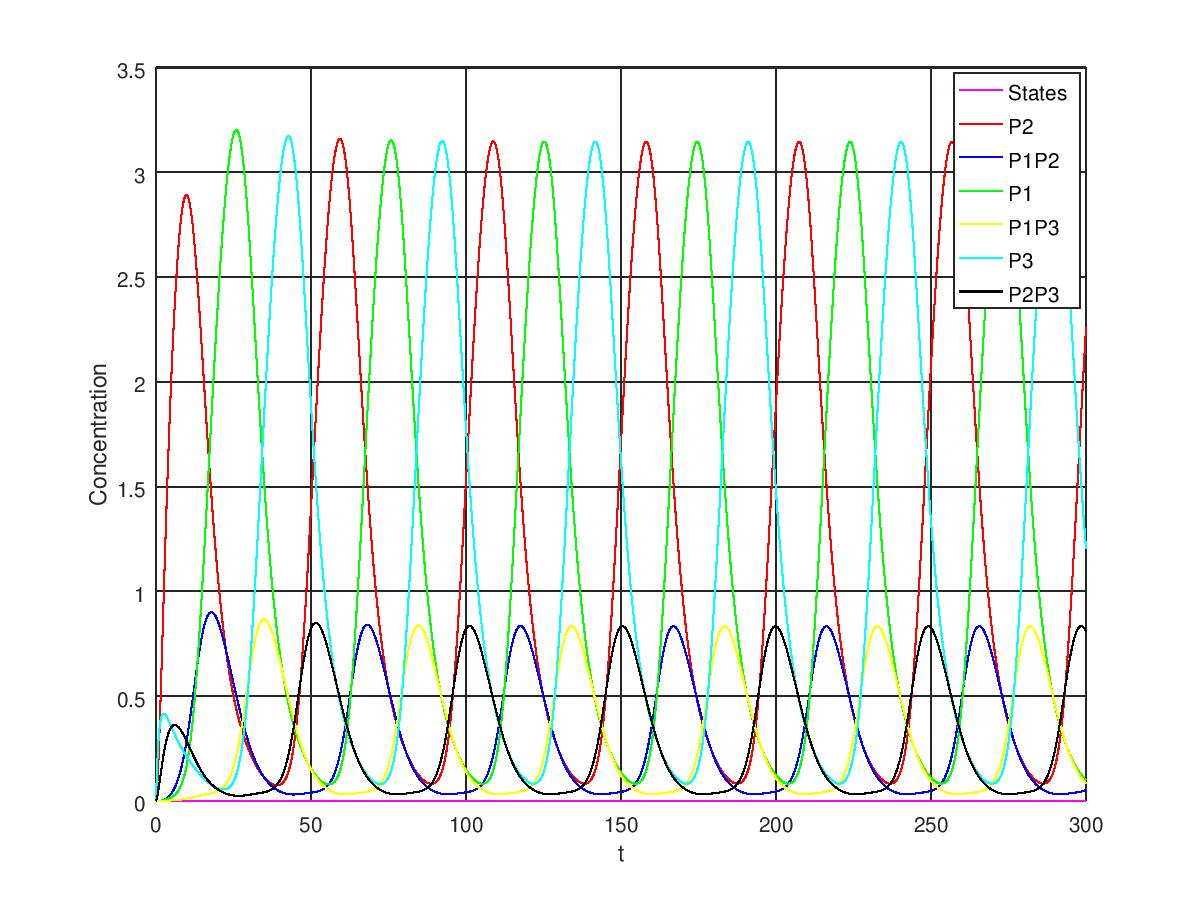
\includegraphics[width=.5\textwidth]{repressilator.jpg}
\caption{Repressilator}
\label{fig:repressilator}
\end{figure}

\subsection{Extracting behavior from Gro}

\begin{center}
    \begin{figure}[h]
        
        % \begin{subfigure}
        %     \includegraphics[scale = 0.4]{p}
        %     \caption{Caption1}
        %     \label{fig:subim1}
        % \end{subfigure}
        
        % \begin{subfigure}[b]{0.3\textwidth}
        %     \includegraphics[scale = 0.25]{p2_plot-inc.eps}
        %     \caption{$B$}
        % \end{subfigure}
        % \begin{subfigure}[b]{0.3\textwidth}
        %     \includegraphics[scale = 0.25]{p3_plot-inc.eps}
        %     \caption{$C$}
        % \end{subfigure}
        
    
        Behaviour of the proteins in the repressilator model simulations using Gro. \textbf{A)} representations of $p_{1}$ protein where the average mean of the many simulations is highlighted in red. \textbf{B)} Representation of the $p2$ protein is shown in cyan plotted from the results of the simulations and is highlighted in green the mean taken of all values portrait by the $dts$ points over the abscissa line. \textbf{C)} Representation of the $p3$ protein achieved, the average mean of values is hightlighted in yellow representing the mean of behaviour from the oscillations expected.
    \end{figure}
\end{center}

A simulation with Gro is particularly interesting, taken that it is the only stochastic simulation used in this research to represent the oscillatory model. The simulation helps greatly in identifying the core representative structure that describes multiple behaviours over different levels of descriptions. Nevertheless, SBML is a model of illustration that facilitates a realistic presentation of such models, giving easy reaction descriptions and featuring a community that provides models in cellular organisms. However, there are limitations in how large cellular circuits can be built with most models showing great behaviour from a mathematical point of view but cannot be fully reproduced in a microbiology laboratory.

As seen in the conversion from a Gro algorithm to SBML model, the Gro reactions is constructed using a rate in which the reactions occur, not ignoring the reaction speed but implicit inside its derivative form, but indifferently from an mathematical language, like octave or mat lab, its stochastic simulation works from a discrete point of view, therefore, you can not have half a reaction occurring, making concentrations of variables always an integer. Obviously, something to elevate from this type of simulation is the non-deterministic results, one of a probabilistic conduct, leading us to use multiple consecutive simulations to understand the behaviour taken from such model.

There are many problems encountered in the process of simulation, one of which is the use of highly miss directing $\delta{t}$ values that can influence the results reached, high value can represent incredibly fast and imprecise simulations, while low values can obtain slow models that could differ from the model described by the algorithm, since the reproduction of an experiment aggregates trustworthy, the values used for the reproduction of such simulations is using $\delta{t}$ = $0.0001$, print of concentrations every $0.001\delta{t}$ in the time scale, with initial concentration and parameters for the oscillations is presented in the mathematical model of the represselator.

The amount of simulations used in the mean average was ten, with the objective to extract the habits of this model, it can be observed the the mean of all simulations on some particular points is far from both stability points of the model, the use of Gro with the varieties of the frequency of the clock, all values are either close to its low concentration level or its high level stability, although, because some fraction of then suffers from a occasionally postpones, with time the mean tends to stabilise somewhere in the middle of of the stability points even if it is impossible for the concentrations to do the same.

\subsection{Simulating output on COPASI}
    \lipsum[1]

\section{Conclusion}
    \lipsum[1]
    
% Topics:
%       => It would be nice if SBML were to be upgraded to fit multicellular models
%       => Then we could extend the parser's syntax to make Gro the multicellular systems biology %              programming language
\section{Future works}
    As it is now, there isn't a multicellular systems biology programming language. The authors believe nonetheless, that Gro could be that language, if only a model exchange format such as SBML were to handle it. After that's done, extending the parser's syntax even without the help of APIs in the likes of libSBML and Tellurium, would be a relatively simple task.

% References
\bibliographystyle{sbc}
\bibliography{sbc-template}

\end{document}
